\documentclass{article}
\usepackage[utf8]{inputenc}
\usepackage[margin=3.0cm]{geometry}
\usepackage{minted}
\usepackage{amssymb}
\usepackage{amsthm}
\usepackage{amsmath}
\usepackage{graphicx}

\pdfinfo{
/Title (Assigment1)
/Author (Felipe Salvatore)}
\setcounter{secnumdepth}{0}  


\title{Assigment 1}
\author{Felipe Salvatore\\
\texttt{felipessalvador@googlemail.com}}
\begin{document}
\maketitle
\textbf{1a)} For any $n$-dimensional vector $x$ an any constant $c$, $softmax(x +c) = softmax(x)$. Where $x+c = (x_1 +c,\dots,x_n +c)$.

\begin{align*}
softmax(x_i +c) & = \frac{e^{(x_{i}+c)}}{\sum_{j=1}^{n} e^{(x_j + c)}} \\
& = \frac{e^{x_{i}}e^{c}}{\sum_{j=1}^{n} e^{x_j}e^{c}}\\
& = \frac{e^{x_{i}}e^{c}}{e^{c}\sum_{j=1}^{n} e^{x_j}}\\
& = \frac{e^{x_{i}}}{\sum_{j=1}^{n} e^{x_j}}\\
& = softmax(x_i)\\ \; .
\end{align*}


\textbf{1b)}

\begin{minted}{python}
def softmax(x):
    # ## YOUR CODE HERE
    if type(x[0]) != np.ndarray:
        x = x.reshape((1, len(x)))
    all_constants = - np.amax(x, axis=1)
    x = x+all_constants[:, np.newaxis]
    x = np.exp(x)
    all_sums = np.sum(x, 1)
    all_sums = np.power(all_sums, -1)
    y = x*all_sums[:, np.newaxis]
    # ## END YOUR CODE
    return y
\end{minted}

\textbf{2a)} Let $\sigma(x) = \frac{1}{1+e^{-x}}$. So, 
\begin{align*}
\frac{\partial \sigma}{\partial x} & = \frac{\partial}{\partial x}\frac{1}{1+e^{-x}} \\
& =\frac{\partial }{\partial x}(1+e^{-x})^{-1} \\
& = -1 (1+e^{-x})^{-2}e^{-x} -1\\
& = \frac{e^{-x}}{(1+e^{-x})^{2}}\\
& = \frac{1}{(1+e^{-x})}\frac{e^{-x}}{(1+e^{-x})}\\
& = \frac{1}{(1+e^{-x})}\frac{(1+e^{-x}) -1}{(1+e^{-x})}\\
& = \frac{1}{(1+e^{-x})}(1 - \frac{1}{(1+e^{-x})})\\
& = \sigma(x)(1 - \sigma(x)) \; .
\end{align*}

\vspace{0.5cm}

Before we continue, let us take a look in the model. Let $D_x,H,D_y \in  \mathbb{N}$ (all greater than $0$), $x \in \mathbb{R}^{D_x}$, $y \in \mathbb{R}^{D_y}$ (an one-hot vector), $b^{1} \in \mathbb{R}^{H}$, $b^{2} \in \mathbb{R}^{D_{y}}$, $W^{1} \in \mathbb{R}^{D_x,H}$ and $W^{2} \in \mathbb{R}^{H,D_y}$. Figure \ref{neural} gives us a visual representation of the model. 

 \begin{figure}
\begin{center}
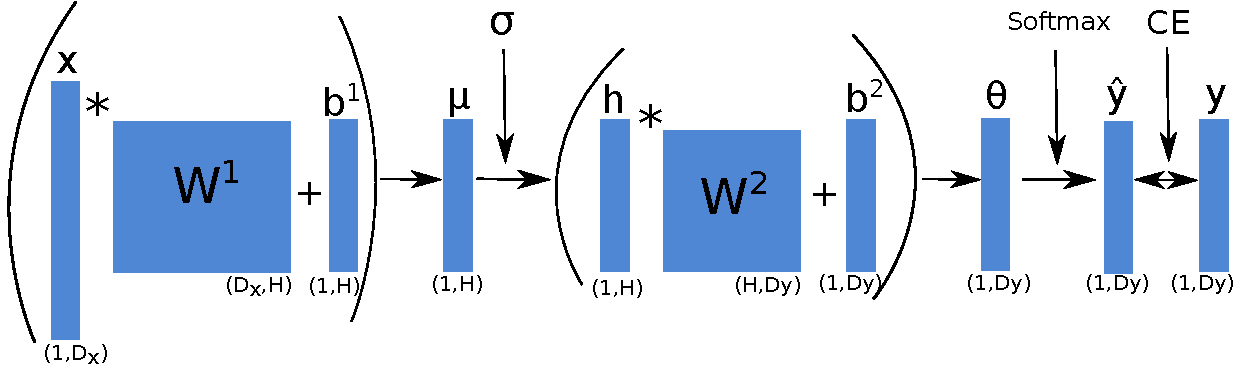
\includegraphics[scale=0.85]{neural.pdf}
\end{center}
\caption{A two layers neural network}
\label{neural}
\end{figure}
To be more formal, we can define all variables in the figure as:
 \begin{equation}\label{eq:1}
\mu_i = \sum_{s=1}^{D_{x}}W^{1}_{si} x_{s} + b^{1}_{i}  \; {\small \text{ with }i = 1, \dots, H}
\end{equation}
\begin{equation}\label{eq:2}
h_i = \sigma(\mu_i)  \; {\small \text{ with }i = 1, \dots, H}
\end{equation}
\begin{equation}\label{eq:3}
\theta_j = \sum_{s=1}^{H}W^{2}_{sj} h_{s} + b^{2}_{j} \;\; {\small \text{ with }j = 1, \dots, D_{y}}
\end{equation}
\begin{equation}\label{eq:4}
\hat{y}_j = softmax(\theta_j) \;\; {\small \text{ with }j = 1, \dots, D_{y}}
\end{equation}
\begin{equation}\label{eq:5}
J(y,\hat{y}) = CE(y,\hat{y}) = -\sum_{s=1}^{D_{y}} y_s  \log(\hat{y}_s)
\end{equation}
where CE stands for \textit{cross-entropy}. Let $k$ be the only index in ${1,\dots,D_{y}}$ such that $y_k =1$. So, equation (\ref{eq:5}) can be simplified as 

\begin{equation}\label{eq:6}
J(y,\hat{y}) = - \theta_k + \log(\sum_{j^{\prime}=1}^{n} e^{\theta_{j^{\prime}}})
\end{equation}

Now we will take all the relevant derivatives.\\

\textbf{2b)} First, for $j = 1, \dots, D_{y}$:
\begin{align*}
\frac{\partial J(y,\hat{y})}{\partial \theta_j}  & = \frac{\partial}{\partial \theta_j}(- \theta_k + \log(\sum_{j^{\prime}=1}^{n} e^{\theta_{j^{\prime}}})) \\
& = - t_j + \frac{\partial}{\partial \theta_j}\log(\sum_{j^{\prime}=1}^{n} e^{\theta_{j^{\prime}}}) \\
& = - t_j + \frac{1}{\sum_{j^{\prime}=1}^{n} e^{\theta_{j^{\prime}}}}\frac{\partial}{\partial \theta_j} e^{\theta_{j}} \\
& = - t_j + \frac{e^{\theta_{j}}}{\sum_{j^{\prime}=1}^{n} e^{\theta_{j^{\prime}}}}\\
& = softmax(\theta_{j}) - t_j \; ,
\end{align*}
where $t_j = 1$ if $j=k$ and $t_j = 0$ otherwise. Thus,
\begin{equation}\label{eq:7}
\frac{\partial J(y,\hat{y})}{\partial \theta_j} = \hat{y}_{j} - y_{j} \; .
\end{equation}


\textbf{2c)}

\textbf{2d)}

\textbf{2e)}

\textbf{2f)}

\textbf{2g)}


\end{document}
